\documentclass[crop,tikz,border=10px,convert=pdf2svg,multi=false]{standalone}
\usetikzlibrary{shapes,arrows,positioning,matrix,decorations,calc}
\begin{document}
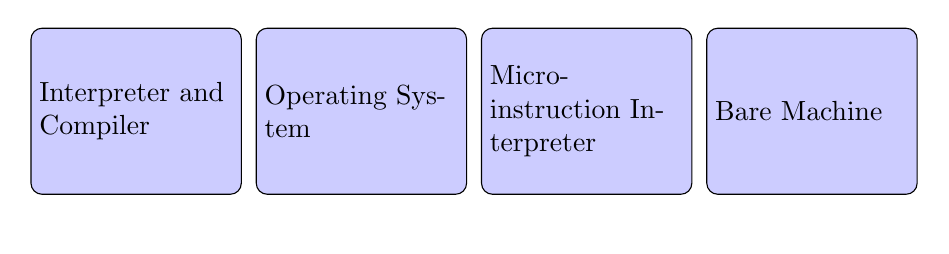
\begin{tikzpicture}[
  every node/.style = {rectangle, draw, rounded corners, fill=blue!20, text
    width=7em, node distance=0.5em, inner sep=.3em, minimum
    height=6em},
  bogus/.style = {minimum height=0, draw=none, fill=none, }]

  \node (app) {Interpreter and Compiler};
  \node[right=of app] (sys) {Operating System};
  \node[right=of sys] (micro) {Micro-instruction Interpreter};
  \node[right=of micro] (hardware) {Bare Machine};

  \node[bogus, below=of app] (left) {};
  \node[bogus, below=of hardware] (right) {};

  \draw[->=stealth,white,line width=.2em] (left.north west) -- (right.north east);

\end{tikzpicture}
\end{document}
